\subsection{Standard Template Library a C++-ban. Tárolók. Bejárók. Algoritmusok. Függvényobjektumok.}

\textbf{STL -- Standard Template Library:}
\begin{itemize}
    \item konténerek: adatstruktúrák
    \item iterátorok: adattárolók elemeinek elérése
    \item algoritmusok: alapvető algoritmusok megvalósítása (sorba rakás, keresés, stb)
\end{itemize}

\begin{center}
    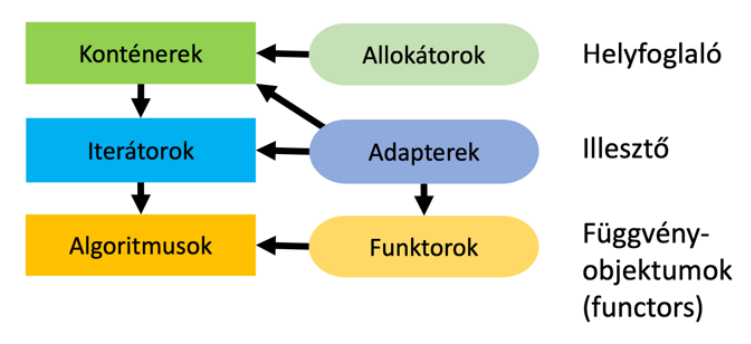
\includegraphics[width=0.7\textwidth]{res/imgs/info_15_stl_structure.png}
\end{center}

\textbf{Tárolók csoportosítása:}
\begin{multicols}{2}
\textbf{Soros}
\begin{itemize}
    \item \texttt{vector<>}
    \item \texttt{array<>} (C++11)
    \item \texttt{deque<>} 
    \item \texttt{forward\_list<>} (C++11)
    \item \texttt{list<>}
\end{itemize}
Az elemek sorrendjét a tárolás sorrendje határozza meg.

\columnbreak

\textbf{Asszociatív} \newline
(Rendezett és Nem rendezett (C++11))
\begin{itemize}
    \item \texttt{set<>}, \texttt{unordered\_set<>}
    \item \texttt{multiset<>}, \texttt{unordered\_multiset<>}
    \item \texttt{map<>}, \texttt{unordered\_map<>}
    \item \texttt{multimap<>}, \texttt{unordered\_multimap<>}
\end{itemize}
Az adatokat egy kulccsal azonosítva tárolják.
\end{multicols}

\textbf{Soros és asszociatív tárolók tulajdonságai:}
\begin{itemize}
    \item van default és copy konstruktora, $=$ operátora
    \item \texttt{a.swap(b)} tagfüggvénye illetve \texttt{swap(a,b)} algoritmusa
    \item $==$ és $!=$ operátora (elemek azonos sorrendben)
    \item sorrendiséget az első nem azonos elem határozza meg
    \item \texttt{begin()} -- bejáró a kezdetre (\texttt{rbegin()} -- kétirányú)
    \item \texttt{end()} -- bejáró a végére (\texttt{rend()})
    \item \texttt{size()} -- méret
    \item \texttt{empty()} -- üres?
    \item \texttt{maxsize()} -- maximálisan tárolható elem
    \item tagok tagfüggvények elérése: \texttt{->}
\end{itemize}

\textbf{Vector:}
\begin{itemize}
    \item elemek sorban (dinamikus tömbökkel megvalósítva)
    \item folytonos adatterület
    \item pointerrel és bejáróval (iterátor) is bejárható
    \item automatikusan növekszik és csökken a tárolási mérete
    \item elemek könnyen elérhetők pozícióval: $\mathcal{O}(1)$
    \item elemek könnyen illeszthetők/törölhetők a végéről: $\mathcal{O}(1)$
    \item elemek beilleszthetők és törölhetők is, de más tárolók erre jobb időt produkálnak
    \item memóriaremodell:
\end{itemize}
\begin{center}
    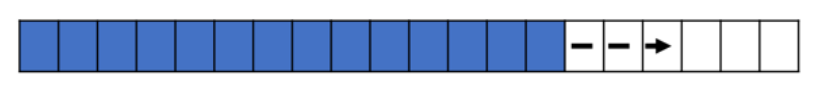
\includegraphics[width=0.8\textwidth]{res/imgs/info_15_vector.png}
\end{center}

\textbf{Array:}
\begin{itemize}
    \item C típusú tömb osztályba foglalása C++11-ben
    \item létrehozás: \texttt{array<típus, méret>}
    \item elemek sorban meghatározott elemszámmal foglalnak helyet
    \item folytonos adatterületen
    \item pointerrel és bejáróval is bejárható
    \item elemek könnyen elérhetők pozícióval: $\mathcal{O}(1)$
    \item elemek lineáris idővel bejárhatók
    \item memóriaremodell:
\end{itemize}
\begin{center}
    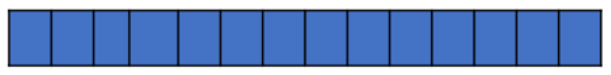
\includegraphics[width=0.8\textwidth]{res/imgs/info_15_array.png}
\end{center}

\begin{itemize}
    \item előnye a hagyományos tömbbel szemben, hogy ez rendelkezik bejáróval, tagfüggvényekkel, valamint alkalmazhatóak rá az algoritmusok
\end{itemize}

\textbf{Deque:}
\begin{itemize}
    \item kétvégű sor
    \item végeiről konstans idővel elem eltávolítása/hozzáadása: \texttt{push\_front(val)}, \texttt{pop\_front()}
    \item nem folytonos adatterületen helyezkedik el
    \item egydimenziós tömböt tartalmazó listában tárolódik
    \item elemek könnyen elérhetők pozíció alapján
    \item az elemek sorban bejárhatók -- iterátorral
    \item lassabb, mint a sor (queue)
    \item memóriaremodell:
\end{itemize}
\begin{center}
    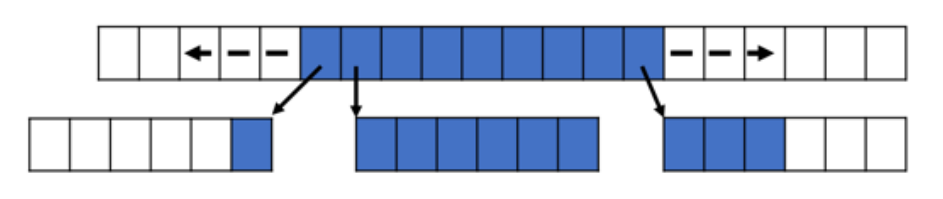
\includegraphics[width=0.8\textwidth]{res/imgs/info_15_deque.png}
\end{center}

\textbf{Egyirányú láncolt lista -- forward\_list:}
\begin{itemize}
    \item csak az elején lehet bővíteni: \texttt{push\_front(val)}
    \item elemek nem elérhetők az indexelés operátorral (nincs \texttt{[]} és \texttt{at()})
    \item tetszőleges pozícióba beszúrhatunk/törölhetünk: \texttt{insert\_after()}, \texttt{erase\_after()}
    \begin{itemize}
        \item konstans idő alatt
    \end{itemize}
    \item a beszúrás és törlés művelet nem rontja el az iterátorokat
    \item memóriaremodell:
\end{itemize}
\begin{center}
    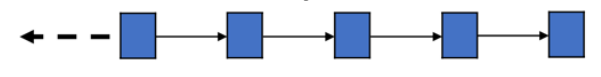
\includegraphics[width=0.6\textwidth]{res/imgs/info_15_forward_list.png}
\end{center}

\textbf{Kétirányban láncolt lista -- list:}
\begin{itemize}
    \item mindkét végéhez hozzáadhatunk, törölhetünk elemet
    \begin{itemize}
        \item \texttt{push\_front(val)}, \texttt{pop\_front()}
        \item \texttt{push\_back(val)}, \texttt{pop\_back()}
    \end{itemize}
    \item elemek nem elérhetők az indexelés operátorral (nincs \texttt{[]} és \texttt{at()})
    \item tetszőleges pozícióba beszúrhatunk/törölhetünk: \texttt{insert()}, \texttt{erase()}
    \begin{itemize}
        \item konstans idő alatt
    \end{itemize}
    \item a beszúrás és törlés művelet nem rontja el az iterátorokat
    \item memóriaremodell:
\end{itemize}
\begin{center}
    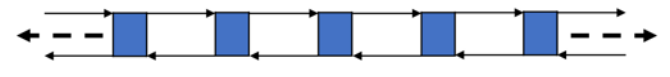
\includegraphics[width=0.6\textwidth]{res/imgs/info_15_list.png}
\end{center}

\textbf{Asszociatív tárolók:}
\begin{itemize}
    \item hozzáférés nem pozíció, hanem egy kulcs értéke alapján történik
    \item rendezett konténer esetén a műveletek általában logaritmikus végrehajtási idejűek
    \item minden lehetséges kulcsérték legalább egyszer előfordul
    \item léteznek kulcsismétlést megengedő változatok (keresés lineáris idejű)
\end{itemize}

\textbf{Set:}
\begin{itemize}
    \item tárolt adatokat kulcsként használja
    \item \texttt{set}: egyedi kulcsok
    \item \texttt{multiset}: ismétlődhetnek a kulcsok
    \item tárolása bináris faként történik
\end{itemize}
\begin{center}
    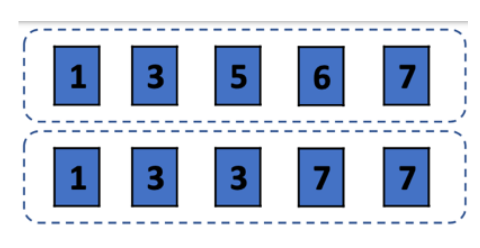
\includegraphics[width=0.7\textwidth]{res/imgs/info_15_set_array.png}
\end{center}
\begin{center}
    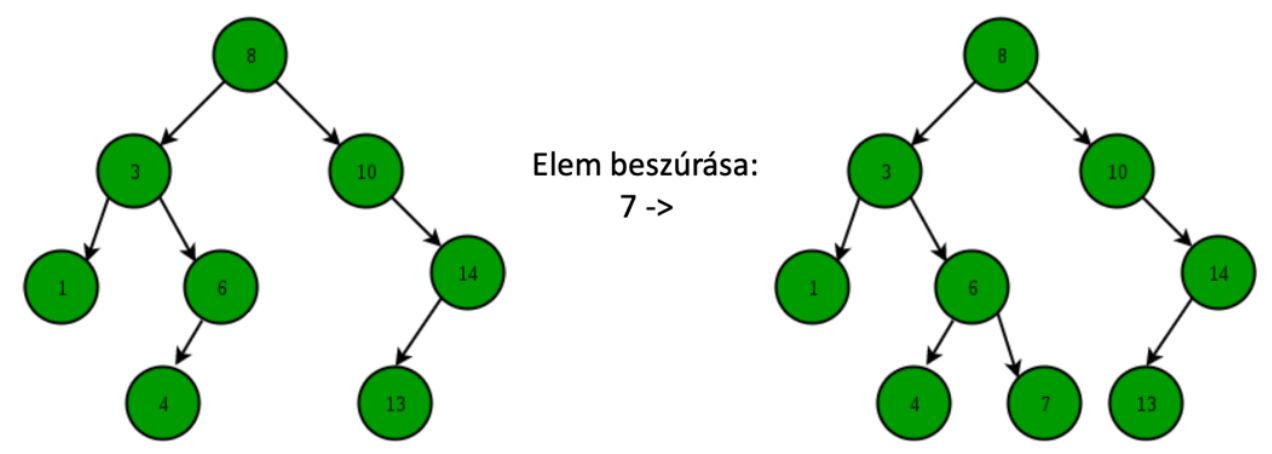
\includegraphics[width=0.9\textwidth]{res/imgs/info_15_set_tree.png}
\end{center}

\textbf{Map:}
\begin{itemize}
    \item adatpárok tárolódnak
    \item \texttt{first} -> kulcs
    \item \texttt{second} -> adat
    \item a map elemei kulcs alapján rendezettek:
    \item \texttt{multimap}: kulcsismétlés megengedett:
\end{itemize}
\begin{center}
    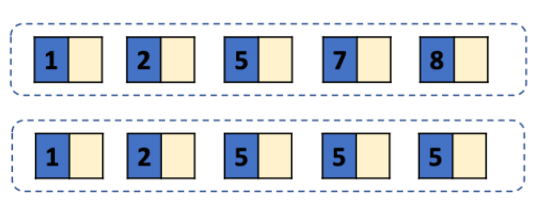
\includegraphics[width=0.5\textwidth]{res/imgs/info_15_map.png}
\end{center}

\textbf{Rendezetlen asszociatív tárolók:}
\begin{itemize}
    \item \texttt{unordered\_set}, \texttt{unordered\_map}
    \item az elemeket egy hasító függvény alapján osztják szét halmazokra
    \item az elemeket a hasító tábla alapján érjük el
\end{itemize}

\textbf{Tároló adapterek:}
\begin{itemize}
    \item soros tárolókra épülő sablonok
    \item nem lehet bejárni őket
    \item nem alkalmazhatók rajtuk algoritmusok
\end{itemize}

\textbf{Stack:}
\begin{itemize}
    \item LIFO: Last In First Out
    \item \texttt{back()}, \texttt{push\_back()}, \texttt{pop\_back()} műveletekkel rendelkező tárolókra adaptálható
\end{itemize}
\begin{center}
    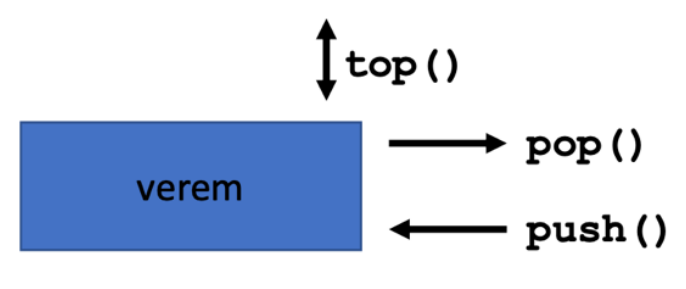
\includegraphics[width=0.5\textwidth]{res/imgs/info_15_stack.png}
\end{center}

\textbf{Queue:}
\begin{itemize}
    \item FIFO: First In First Out
    \item \texttt{front()}, \texttt{back()}, \texttt{push\_back()}, \texttt{pop\_front()} műveletekkel rendelkező tárolókra adaptálható
    \item alapműveletek mindegyikéhez konstans idő szükséges
\end{itemize}
\begin{center}
    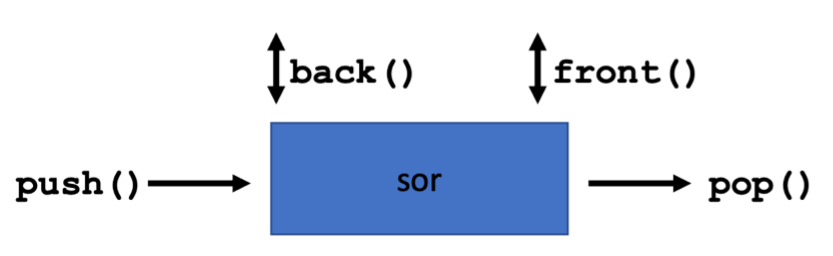
\includegraphics[width=0.6\textwidth]{res/imgs/info_15_queue.png}
\end{center}

\textbf{Priority queue:}
\begin{itemize}
    \item BIFO: Best In First Out -- legjobb a legnagyobb prioritású elem
    \item \texttt{vector}, \texttt{deque} konténerekre adaptálható
    \item az elsőbbséget egy rendezési előírás definiálja
    \item a sor elején mindig a legnagyobb prioritású elem helyezkedik el
\end{itemize}
\begin{center}
    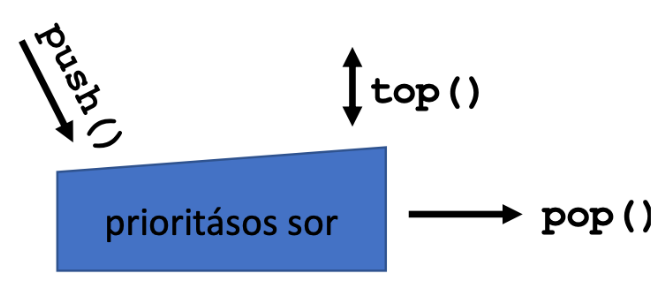
\includegraphics[width=0.6\textwidth]{res/imgs/info_15_priority_queue.png}
\end{center}

\textbf{Iterátorok:}
\begin{itemize}
    \item adathalmaz bejárására alkalmas objektumok
    \item egy pozíciót határoz meg a tárolóban
\end{itemize}

\textbf{Algoritmusok:}
\begin{itemize}
    \item globális függvénysablonok, iterátorok segítségével férnek hozzá a tárolt adatokhoz
    \item függetlenek a konténerektől, az iterátorok feladata ismerni a konténert
    \item ha a tároló valamilyen algoritmust saját tagfüggvénnyel is meg tud valósítani, célszerűbb azt használni (hatékonyabb és biztonságosabb)
    \item a végrehajtott algoritmus működési eredményét többféleképpen is megkaphatjuk:
    \begin{itemize}
        \item konténerben
        \item iterátorként
        \item adatként
    \end{itemize}
    \item \textbf{nem módosító} algoritmusok (nem változtatják meg az elemeket, se azok sorrendjét):
    \begin{itemize}
        \item \texttt{equal()}, \texttt{find()}, \texttt{for\_each()}, \texttt{max()}, \texttt{min()}, \texttt{mismatch()}, \texttt{search()}
    \end{itemize}
    \item \textbf{módosító} algoritmusok:
    \begin{itemize}
        \item \texttt{copy()}, \texttt{fill()}, \texttt{for\_each()} (attól függ, mit csinálsz vele), \texttt{merge()}, \texttt{move()}, \texttt{replace()}, \texttt{swap()}, \texttt{transform()}
        \item \textbf{eltávolító} algoritmusok:
        \begin{itemize}
            \item \texttt{remove()}, \texttt{unique()}
        \end{itemize}
        \item \textbf{átalakító} algoritmusok (elemsorrend megváltoztatása):
        \begin{itemize}
            \item \texttt{partition()}, \texttt{reverse()}, \texttt{rotate()}
        \end{itemize}
        \item \textbf{rendező} algoritmusok:
        \begin{itemize}
            \item \texttt{partition()}, \texttt{sort()} 
        \end{itemize}
    \end{itemize}
    \item \textbf{rendezett tartomány} algoritmusai:
    \begin{itemize}
        \item \texttt{binary\_search()}, \texttt{equal\_range()}, \texttt{lower\_bound()}, \texttt{upper\_bound()}, \texttt{merge()}
    \end{itemize}
\end{itemize}

\textbf{Függvényobjektumok:}
\begin{itemize}
    \item algoritmusok működése testre szabható
    \item meghatározhatjuk, milyen művelet hajtódjon végre az elemeken
    \item hagyományos függvény mutató is lehet, de legtöbbször objektum
    \item olyan osztály, mely megvalósítja a függvényhívás \texttt{()} operátorát:
\begin{minted}{cpp}
típus operator() (paraméterek) { }
\end{minted}
    \item létezik egyoperandusú és kétoperandusú
    \item hívásakor az osztály példányát (objektumát) adjuk át
    \item előre definiált függvényobjektumok:
\end{itemize}

\begin{multicols}{2}
\textbf{Aritmetikai műveletek}
\begin{itemize}
    \item \texttt{negate}: \texttt{- param}
    \item \texttt{plus}: \texttt{param1 + param2}
    \item \texttt{minus}: \texttt{param1 - param2}
    \item \texttt{multiplies}: \texttt{param1 * param2}
    \item \texttt{divides}: \texttt{param1 / param2}
    \item \texttt{modulus}: \texttt{param1 \% param2}
\end{itemize}

\columnbreak

\textbf{Összehasonlítások}
\begin{itemize}
    \item \texttt{equal\_to}: \texttt{param1 == param2}
    \item \texttt{not\_equal\_to}: \texttt{param1 != param2}
    \item \texttt{less}: \texttt{param1 < param2}
    \item \texttt{greater}: \texttt{param1 > param2}
    \item \texttt{less\_equal}: \texttt{param1 <= param2}
    \item \texttt{greater\_equal}: \texttt{param1 >= param2}
\end{itemize}
\end{multicols}